\chapter{Elgendiho referenční algoritmus}
\label{chap:elgendi_neurokit}

Tato kapitola popisuje, jak lze ve fotopletysmografickém (\acs{PPG}) signálu nalézt systolické vrcholy s využitím Elgendiho algoritmu, který je implementován v~knihovně NeuroKit2.
NeuroKit2 reaguje na \uv{krizi reprodukovatelnosti} v psychologii a neurovědách a nabízí open-source kód, strukturovanou dokumentaci i podporu k začleňování funkcí přímo do výzkumných prací~\cite{NeuroKit2}.
Knihovna je dostupná na \url{https://github.com/neuropsychology/NeuroKit} (zdrojový kód) a \url{https://neurokit2.readthedocs.io/} (dokumentace) a její návrh umožňuje průběžný vývoj a modifikace.
V~kapitole~\ref{chap:PPG_teorie} byly již podrobně shrnuty principy \acs{PPG}, proto se zde zaměříme na samotnou detekci vrcholů a její realizaci.

\section{Obecná struktura algoritmu}
Algoritmus se skládá z několika kroků: \emph{filtrace} pomocí pásmové propusti, \emph{umocnění} signálu, vytvoření dvou \emph{klouzavých průměrů} a dvou \emph{prahů}, jak je zobrazeno na obrázku~\ref{fig:alg-scheme}~\cite{Elgendi2013}.
Vstupem je surový fotopletysmografický záznam, zatímco výstupem jsou konkrétní časové pozice nalezených systolických vrcholů.

\begin{figure}[htbp]
	\centering
	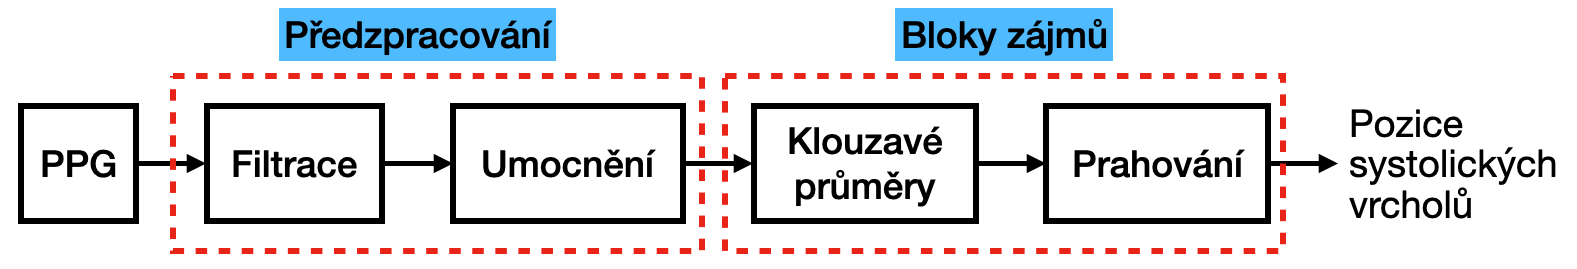
\includegraphics[width=1\textwidth]{./obrazky/ElgendiBlokSchema.png}
	\caption[Struktura Elgendiho algoritmu]{Zjednodušené schéma Elgendiho algoritmu~\cite{Elgendi2013}.}
	\label{fig:alg-scheme}
\end{figure}

\section{Předzpracování signálu}
Před samotnou detekcí je vhodné potlačit šum a odstranit pomalé změny amplitudy.
Elgendi~\cite{Elgendi2013} používá druhý řád Butterworthova filtru se zpracováním v~přímém i reverzním směru (tzv.~filtrace s nulovým fázovým posuvem).
Frekvenční charakteristika filtru byla nastavena na pásmo 0,5--8~Hz, což postačuje pro typické PPG kmitočty a dostatečně potlačí pásmový posun i vyšší frekvence nesouvisející se systolickými vrcholy.

Na obrázku~\ref{fig:filter-example} je ukázka amplitudové charakteristiky a zfiltrovaného úseku signálu.

\begin{figure}[htbp]
	\centering
	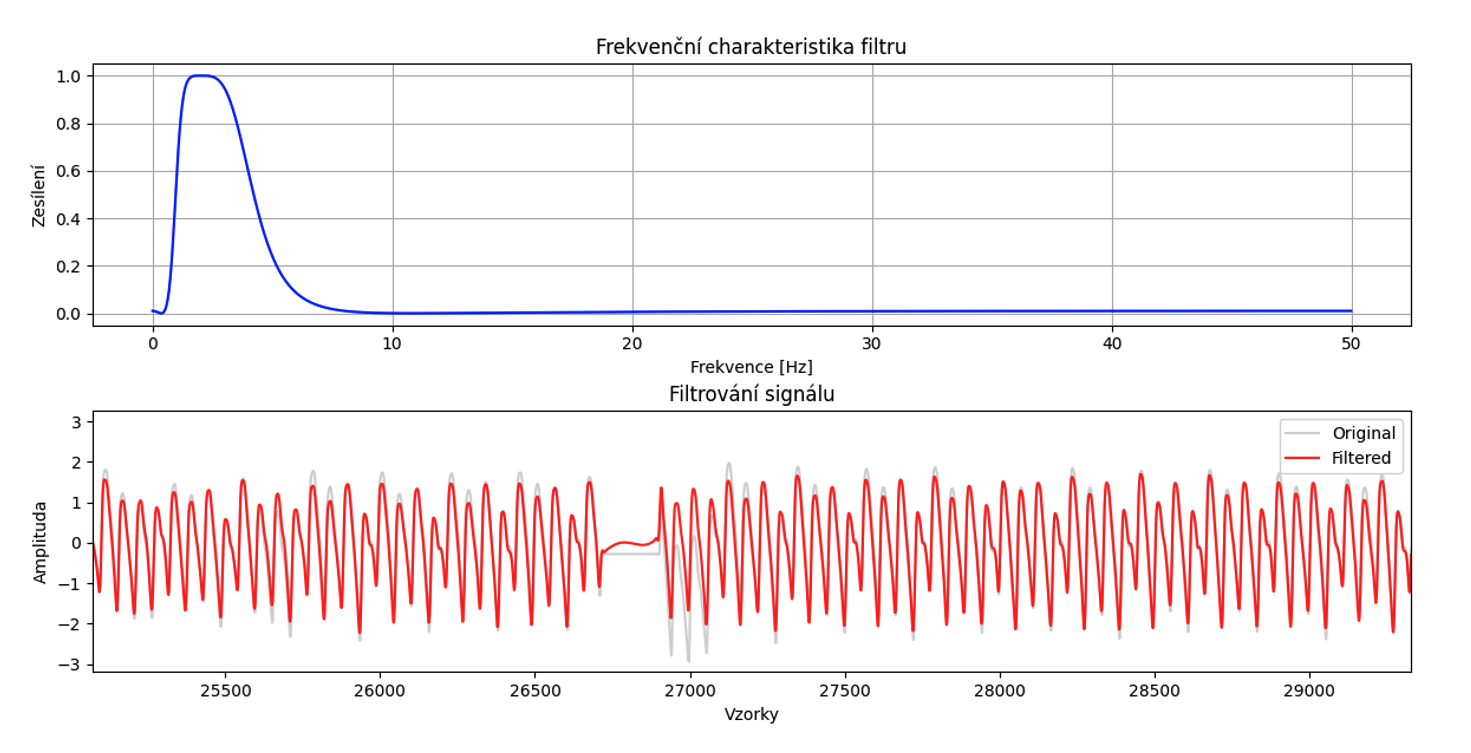
\includegraphics[width=0.8\textwidth]{./obrazky/ElgendiBandpass.png}
	\caption[Filtrace PPG signálu]{Horní graf: příklad amplitudové přenosové charakteristiky pásmové propusti. Dolní graf: znázornění filtrace PPG (šedě původní signál, červeně po filtraci).}
	\label{fig:filter-example}
\end{figure}

Po filtraci se signál umocňuje na druhou, aby se zdůraznily rozdíly mezi systolickou vlnou a ostatními složkami (například diastolickými zářezy).
Výsledná hodnota $y[n]$ po umocnění je:
\begin{equation}
	y[n] = Z[n]^2,
	\label{eq:square}
\end{equation}
kde $Z[n]$ je již vyfiltrovaný signál.
V~důsledku toho bývá systolický vrchol zdůrazněn na úkor diastolických zářezů nebo šumu~\cite{Elgendi2013}, jak je ilustrováno na obrázku~\ref{fig:squared-signal}.

\begin{figure}[htbp]
	\centering
	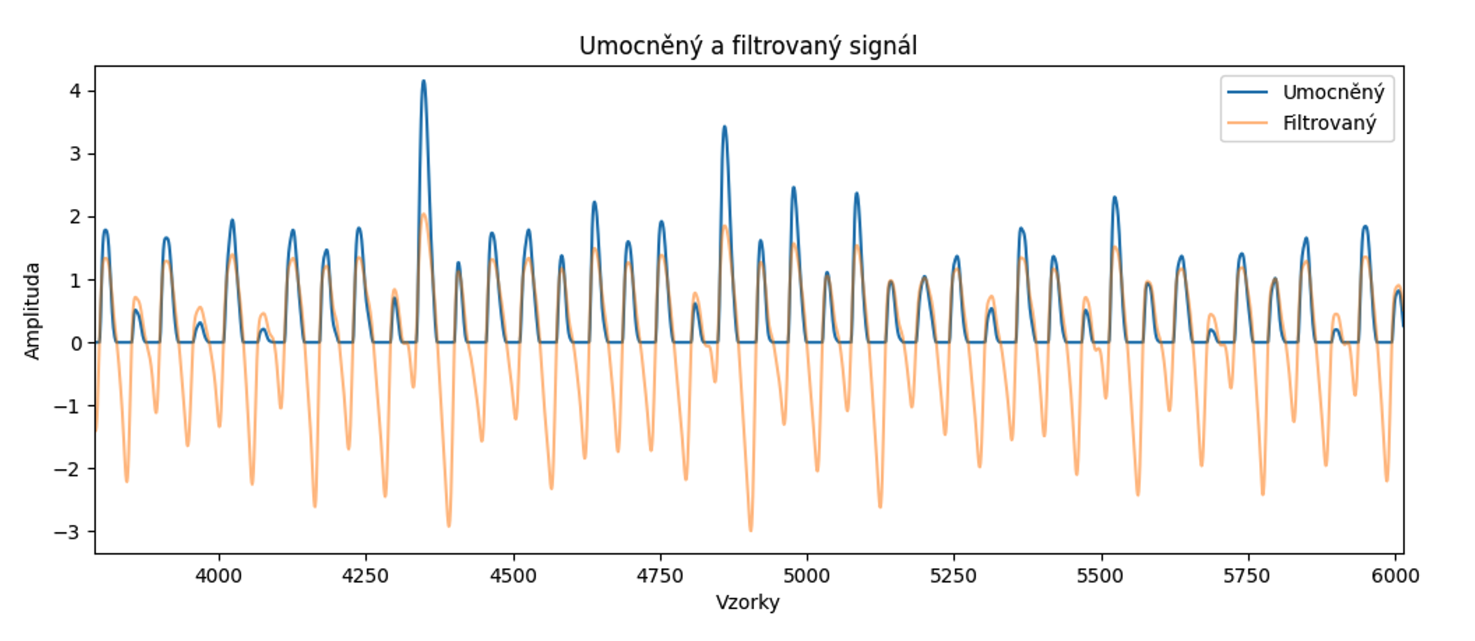
\includegraphics[width=0.8\textwidth]{./obrazky/ElgendiUpravenySignal.png}
	\caption[Umocněný a filtrovaný PPG]{Porovnání filtrovaného umocněného PPG.}
	\label{fig:squared-signal}
\end{figure}

\section{Dvoufázové prahování a nalezení vrcholů}
Po umocnění je potřeba určit, kde přesně hledat potenciální maximum, tedy systolický vrchol.
Pro tento účel využívá Elgendiho algoritmus dva různé klouzavé průměry~(\acs{MA}), které se liší délkou okna a následně dva prahy pro finální detekci vrcholů~\cite{Elgendi2013}.

% Krátké okno prvního klouzavého průměru přibližně odpovídá šířce systolické vlny, zatímco delší okno (druhého průměru) pokrývá délku celého srdečního cyklu.
% Na základě jejich rozdílu a adaptivních prahů se definují \uv{bloky zájmu}, kde by mohl ležet vrchol.
% V takto vymezeném úseku se hledá a bere maximální hodnota jako systolický vrchol.
% Souhrnně lze postup vyjádřit rovnicí

% Elgendiho algoritmus určuje systolické vrcholy dvoustupňovým postupem s~využitím dvou klouzavých průměrů a následného prahování~\cite{Elgendi2013}.
% Nejprve jsou zkonstruovány dva klouzavé průměry, které se liší délkou okna.
\acs{MA_P} zvýrazňuje oblast systolického vrcholu, zatímco \acs{MA_B} reprezentuje průměrnou úroveň v rámci celého tepu~\cite{Elgendi2013}.
Pomocí \acs{MA_B} se definuje první práh \acs{THR_1}, a to přičtením posuvného členu $\alpha$ k \acs{MA_B}, kde $\alpha$ je definována jako $\alpha = \beta\,\overline{z^2}$; v~této formuli je $\beta$ empirická konstanta (např.\ 0,02) a $\overline{z^2}$ střední hodnota umocněného a zfiltrovaného PPG signálu.
Porovnáním \acs{MA_P} s~\acs{THR_1} se identifikují tzv.\ bloky zájmu, které mohou obsahovat systolický vrchol či rušení.

V další fázi se tyto bloky podrobí druhému prahování, aby se odstranily ty, jejichž šířka je nižší, než se očekává pro systolickou vlnu~\cite{Elgendi2013}.
Pokud například platí $\mathrm{THR}_2 = W_1$, kde $W_1$ odpovídá délce systolického pulzu, pak všechny bloky užší než $\mathrm{THR}_2$ se považují za šum a odfiltrují se.
V akceptovaných blocích se následně najde nejvyšší hodnota signálu, která je interpretována jako poloha systolického vrcholu.
Tímto dvoustupňovým přístupem lze eliminovat falešné úseky způsobené diastolickou vlnou či jinými artefakty, a robustně tak určit polohu hlavního vrcholu~\cite{Elgendi2013}.

% \begin{figure}[htbp]
% 	\centering
% 	\includegraphics[width=0.78\textwidth]{blocks_detection.jpg}
% 	\caption[Oblasti hledání vrcholů]{Zobrazení umocněného signálu (tmavě modře), filtrovaného signálu (světle modře) a dvou klouzavých průměrů (zelené křivky). Šedé pruhy znázorňují vybrané úseky (bloky), kde hledáme maximum jako systolický vrchol (červené body).}

% 	\label{fig:block-detection}
% \end{figure}

% Aby se předešlo vícenásobné detekci blízko sebe, zavádí se také minimální vzdálenost mezi detekovanými vrcholy. Tato vzdálenost je obvykle nastavena podle reálné fyziologie, např. 200~ms při klidové tepové frekvenci.

% \section{Integrace do NeuroKit2}
% Popsaný postup je implementován v knihovně NeuroKit2 volbou \verb|method="elgendi"| při volání funkce \verb|ppg_process|:
% \begin{verbatim}
% import neurokit2 as nk

% signals, info = nk.ppg_process(
% 	ppg_signal, sampling_rate=fs,
% 	method="elgendi",
% 	method_quality="templatematch"
% )
% \end{verbatim}
% Výstup \verb|signals| typicky obsahuje sloupec s~pozicemi vrcholů a okamžitými hodnotami TF, zatímco \verb|info| nese další kontextové informace, například seznam indexů vrcholů či parametry filtrace.

% \section{Zhodnocení kvality signálu}
% Metoda \verb|templatematch| porovnává tvar každého detekovaného pulzu s~referenční šablonou a vyhodnocuje, do jaké míry odpovídá typické morfologii PPG. Takový přístup zjišťuje, zda je příslušný úsek skutečně “kvalitní” a nemá výrazné artefakty. Výsledkem může být číselné skóre kvality nebo binární označení (kvalitní / nekvalitní).

% \section{Závěr}
% Elgendiho algoritmus, s~částečnými modifikacemi v NeuroKit2, nabízí robustní a do značné míry automatizované řešení detekce systolických vrcholů v PPG. Díky adaptivním prahům a využití dvou klouzavých průměrů dokáže úspěšně potlačit různé formy šumu a spolehlivě najít systolický vrchol. K~praktickému použití navíc poslouží modul \emph{Template-Matching}, který vyhodnotí důvěryhodnost každého detekovaného pulzu.

